\documentclass{article}
\usepackage{geometry}
\usepackage{graphicx}
\usepackage{hyperref}
\usepackage{listings}
\usepackage{inconsolata}
\usepackage{tikz}
\usepackage{enumitem}

\geometry{a4paper, margin=1in}
\renewcommand{\familydefault}{\sfdefault}

\usetikzlibrary{shapes.geometric, arrows, positioning, fit, calc}

\hypersetup{
    colorlinks=true,
    linkcolor=blue,
    filecolor=magenta,
    urlcolor=cyan,
}

\lstset{
    basicstyle=\small\ttfamily,
    breaklines=true,
    backgroundcolor=\color[rgb]{0.95,0.95,0.95},
    commentstyle=\color{gray},
    keywordstyle=\color{blue},
    stringstyle=\color{red},
    showstringspaces=false,
    frame=single,
    rulecolor=\color{black},
    captionpos=b,
    tabsize=2,
    escapeinside={\%*}{*)},
}

\newcommand{\filepath}[1]{\texttt{\small #1}}

\title{Detailed System Architecture Documentation}
\author{Gemini Agent}
\date{\today}

\begin{document}

\maketitle
\tablecontents
\newpage

\section{System Overview}
This document provides a detailed architecture of the mixed-reality system. The system integrates an Apple Vision Pro (AVP) application with a powerful backend that performs real-time computer vision (CV) tasks. The architecture is designed for robust 6D pose estimation, with special considerations for sensor uncertainty and object occlusion.

\begin{figure}[h!]
\centering
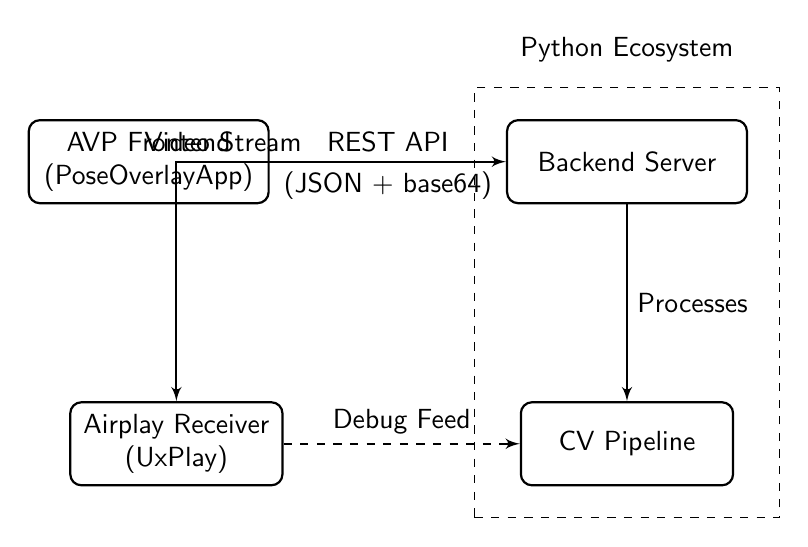
\begin{tikzpicture}[
    node distance=2.5cm and 3cm,
    block/.style={rectangle, draw, thick, text width=6em, text centered, rounded corners, minimum height=3em},
    line/.style={draw, thick, -latex'}
]
    % Nodes
    \node[block, text width=8em] (avp) {AVP Frontend (PoseOverlayApp)};
    \node[block, right=of avp, text width=8em] (backend) {Backend Server};
    \node[block, below=of backend, text width=7em] (pipeline) {CV Pipeline};
    \node[block, left=of pipeline, text width=7em] (airplay) {Airplay Receiver (UxPlay)};

    % Connections
    \path[line] (avp) -- node[above] {REST API} node[below] {(JSON + base64)} (backend);
    \path[line] (backend) -- node[right] {Processes} (pipeline);
    \path[line] (avp) -| node[above, near start] {Video Stream} (airplay);
    \path[line, dashed] (airplay) -- node[above] {Debug Feed} (pipeline);

    % Bounding box for backend
    \node[draw, dashed, inner sep=0.4cm, label={[yshift=0.2cm]above:Python Ecosystem}, fit=(backend) (pipeline)] {};
\end{tikzpicture}
\caption{High-level system architecture showing the interaction between the AVP frontend and the backend services.}
\label{fig:architecture}
\end{figure}

\section{AVP UI (Apple Vision Pro)}
The user interface is a native visionOS application designed to provide an immersive mixed-reality experience.

\subsection{Project Location}
The source code for the application is located at:
\begin{itemize}
    \item \filepath{visionos/PoseOverlayApp/}
\end{itemize}
This directory contains the Xcode project for the \texttt{PoseOverlayApp}.

\subsection{Conceptual Layout}
The UI is responsible for rendering a live video feed from the AVP's cameras and overlaying virtual content, such as the estimated pose of an object, onto the real world.

\begin{figure}[h!]
\centering
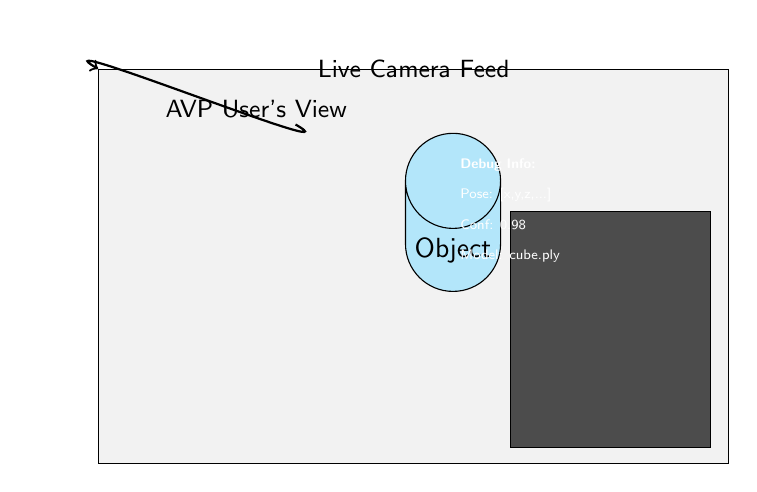
\begin{tikzpicture}[
    screenelem/.style={draw, fill=gray!10, text centered},
    textlabel/.style={font=\sffamily\small}
]
    % Main screen
    \node[screenelem, minimum width=8cm, minimum height=5cm] (screen) at (0,0) {};
    \node[textlabel] at (screen.north) {Live Camera Feed};

    % 3D Overlay
    \node[screenelem, shape=cylinder, shape border rotate=90, minimum width=1cm, minimum height=1.5cm, fill=cyan!30] (overlay) at (0.5, 0.2) {Object};

    % Debug panel
    \node[screenelem, fill=black!70, minimum width=2.5cm, minimum height=3cm, text width=2.3cm, align=left] (debug) at (2.5, -0.8) {};
    \node[textlabel, color=white, align=left] at (debug.north west) {
        \tiny \textbf{Debug Info:}\\
        \tiny Pose: [x,y,z,...]\\
        \tiny Conf: 0.98\\
        \tiny Model: cube.ply
    };

    \node[textlabel] at (-2, 2) {AVP User's View};
    \draw[thick, ->] (-1.5, 1.8) to[out=-30,in=150] (screen.north west);
\end{tikzpicture}
\caption{A conceptual diagram of the \texttt{PoseOverlayApp} user interface, showing the 3D model overlay and a debug information panel.}
\label{fig:ui_concept}
\end{figure}

\section{API Communication (\texttt{main_api.py})}
Communication between the AVP app and the backend is handled by a Flask-based REST API defined in \filepath{backend/main_api.py}. This API serves as the central hub for data exchange.

\subsection{Endpoints}
The API exposes numerous endpoints, grouped by functionality:

\begin{description}[style=multiline,leftmargin=3.5cm]
    \item[\texttt{GET /health}] Health check to confirm the server is running.
    \item[\texttt{GET /stats}] Returns processing statistics from the API and CV pipeline.

    \item[\textbf{CV Data Transfer}]
    \item[\texttt{POST /receive_frame}] Primary endpoint to submit a raw, base64-encoded video frame for processing by the CV pipeline.
    \item[\texttt{GET /rgb_frame}] Retrieves the last raw RGB frame received.
    \item[\texttt{GET /mask}] Retrieves the latest segmentation mask as a base64 image.
    \item[\texttt{GET /depth}] Retrieves the latest depth map.
    \item[\texttt{GET /disparity}] Retrieves the latest disparity map.
    \item[\texttt{POST /external_disparity}] Allows the AVP app to send its own computed disparity map to the backend.

    \item[\textbf{Configuration}]
    \item[\texttt{GET, POST /config}] Get or update the configuration of the underlying CV pipeline (e.g., HSV thresholds).

    \item[\textbf{Head Pose Tracking}]
    \item[\texttt{GET, POST /head_pose}] Endpoints to submit head pose data from the AVP and retrieve the last known head pose. This is crucial for motion compensation.

    \item[\textbf{Model Management}]
    \item[\texttt{GET /models}] Lists all available \texttt{.ply} 3D models in the \filepath{models/} directory.
    \item[\texttt{GET /model}] Retrieves the mesh data for a specific model by name.
    \item[\texttt{POST /select_model}] Sets the active 3D model to be used for pose estimation.

    \item[\textbf{Pose Estimation}]
    \item[\texttt{POST /avp_pose}] A high-level convenience endpoint for the AVP. It accepts all necessary data (RGB, depth, intrinsics), packages it, and forwards it to the core pose estimator. It can also return a mock pose for debugging.
    \item[\texttt{POST /pose}] The core pose estimation endpoint. It can either forward the request to an external, specialized pose API or return a mock pose, depending on the \texttt{use_random_pose} flag.
\end{description}

\section{CV Pipeline (\texttt{computer_vision_pipeline.py})}
The core CV logic is encapsulated in \filepath{backend/full_python_pipeline/computer_vision_pipeline.py}. While this is a complex component, its functionality can be inferred from the API structure.

\subsection{Inferred Pipeline Stages}
\begin{enumerate}
    \item \textbf{Frame Decoding:} Input data (base64 strings) are decoded into OpenCV image formats.
    \item \textbf{Image Pre-processing:} Images are converted to different color spaces (e.g., HSV for color filtering, grayscale for marker detection).
    \item \textbf{Segmentation & Masking:} The region of interest (the object to be tracked) is isolated from the background, generating a binary mask.
    \item \textbf{Feature Detection:} For pose estimation, the system likely uses ArUco markers or other features to find an initial reference point, as suggested by the \texttt{/detected_frame} endpoint.
    \item \textbf{Depth Estimation:} If not provided by the AVP, a depth or disparity map is computed from the video feed, likely using a monocular depth estimation model or stereo vision techniques.
    \item \textbf{Pose Calculation:} Using the 2D location of the object, its corresponding depth data, and the camera intrinsics, the pipeline calculates the 6D pose (rotation and translation) of the object.
    \item \textbf{Pose Refinement:} The initial pose can be corrected using data from the AVP's head tracking, compensating for latency and camera motion.
\end{enumerate}

\section{Advanced Pose Estimation with Data-Driven Control}
The file \filepath{MA/occlusion_approach/files/test_occ_dbc_gp.py} presents a sophisticated simulation for robust 6D pose estimation using a data-driven, model-free approach. This method is designed to handle real-world challenges like sensor noise, tracking drift, and object occlusion.

\subsection{Willems' Data-Driven Control (DDC)}
The core of this method is the \texttt{WillemsDDC} class, which implements a controller based on Willems' Fundamental Lemma. Instead of relying on an explicit mathematical model of the system dynamics, this approach uses a history of past observations and poses to predict future states. It achieves this by constructing Hankel matrices from the historical data and solving a linear system.

\subsection{Occlusion and Uncertainty Handling}
A key feature is its robust handling of uncertainty. The algorithm calculates a \texttt{trust_factor} for each new measurement. This factor is derived from multiple sources:
\begin{itemize}
    \item \textbf{Geometric Occlusion:} Explicit check if the line of sight to the object is blocked.
    \item \textbf{Camera Pose Uncertainty:} Accounts for drift and noise from the SLAM system.
    \item \textbf{Intrinsics Uncertainty:} Models drift in the camera's intrinsic parameters.
\end{itemize}
When the \texttt{trust_factor} is high (low trust), the algorithm discounts the measurement and relies more on its internal prediction.

\subsection{Gaussian Process for Uncertainty Modeling}
The script also uses a \texttt{GaussianProcessRegressor} to model the uncertainty in the object's trajectory over time, further improving the robustness of the estimation.

\end{document}
